% ========================================
% CHƯƠNG 1: TỔNG QUAN ĐỀ TÀI
% ========================================
\chapter{TỔNG QUAN ĐỀ TÀI}
\label{ch:tongquan-detai}

% ----- TÓM TẮT CHƯƠNG -----
\vspace{0.5cm}
\noindent\textit{Chương này trình bày bối cảnh và lý do lựa chọn đề tài xây dựng hệ thống IoT Zigbee Smart Building. Tiếp theo, chương xác định rõ mục tiêu tổng quát, mục tiêu cụ thể, phạm vi nghiên cứu và các giới hạn thực tế của đồ án. Cuối cùng, phương pháp thực hiện, những đóng góp chính về mặt kỹ thuật và cấu trúc tổng thể của báo cáo cũng được khái quát hóa nhằm cung cấp cái nhìn toàn cảnh trước khi đi vào các nội dung kỹ thuật chi tiết.}
\vspace{0.5cm}

% ========================================
% 1.1 BỐI CẢNH VÀ LÝ DO CHỌN ĐỀ TÀI
% ========================================
\section{Bối cảnh và lý do chọn đề tài}
\label{sec:ch1-boicanh}

Trong những năm gần đây, sự phát triển mạnh mẽ của công nghệ mạng không dây và Internet vạn vật (Internet of Things - IoT) đã thúc đẩy việc ứng dụng tự động hóa vào quản lý vận hành tòa nhà. Smart Building (tòa nhà thông minh) không còn là khái niệm lý thuyết mà đã trở thành xu hướng tất yếu nhằm tối ưu hóa lượng điện năng tiêu thụ, nâng cao độ an toàn và mang lại trải nghiệm tiện nghi cho người sử dụng. Trong các hệ thống này, nhu cầu giám sát trạng thái môi trường, phát hiện sự hiện diện của con người và điều khiển các thiết bị phụ tải (như đèn chiếu sáng, công tắc) là những bài toán cốt lõi cần giải quyết.

Đối với mạng kết nối nội bộ (local network) trong tòa nhà, việc sử dụng các công nghệ truyền thông không dây phổ biến như Wi-Fi thường bộc lộ những hạn chế lớn về mặt tiêu thụ năng lượng và khả năng chịu tải của điểm truy cập trung tâm khi số lượng thiết bị lên tới hàng trăm node. Do đó, các công thức truyền thông tiết kiệm năng lượng, hỗ trợ cấu trúc liên kết mạng lưới (mesh network) như Zigbee được xem là giải pháp tối ưu. Zigbee hoạt động trên tiêu chuẩn IEEE 802.15.4, cho phép các thiết bị tự động định tuyến gói tin qua nhau, giúp mở rộng phạm vi phủ sóng mà không yêu cầu công suất phát lớn, đồng thời giảm thiểu đáng kể chi phí duy trì nguồn pin cho các cảm biến.

Tuy nhiên, các mạng Zigbee cục bộ không thể tự kết nối trực tiếp với các ứng dụng di động hoặc hệ thống quản lý từ xa qua mạng IP diện rộng. Điều này đòi hỏi sự xuất hiện của một thiết bị trung gian gọi là Gateway. Thiết bị Gateway đóng vai trò làm cầu nối chuyển đổi giữa giao thức Zigbee RF tầm ngắn và mạng IP (chạy các giao thức như MQTT, HTTP) kết nối lên Cloud. Sự phối hợp giữa Gateway và hệ thống đám mây (Cloud Backend) cho phép lưu trữ lịch sử vận hành, xử lý các kịch bản tự động hóa phức tạp và cung cấp các giao diện lập trình ứng dụng (API) cho ứng dụng di động của người dùng cuối. 

Hơn nữa, các giải pháp smart building thương mại hiện nay thường là các hệ sinh thái đóng (closed ecosystem) của các nhà sản xuất lớn, gây khó khăn cho việc tích hợp thiết bị của bên thứ ba và hạn chế khả năng tùy biến logic điều khiển. Xuất phát từ nhu cầu nghiên cứu một nền tảng quản lý thiết bị mở, có khả năng làm chủ từ firmware thiết bị, logic xử lý tại gateway cho đến kiến trúc cloud backend, đề tài \textbf{"Hệ thống IoT Zigbee Smart Building"} đã được lựa chọn để thực hiện. Đồ án tập trung nghiên cứu thiết kế và tích hợp đồng bộ các lớp thiết bị, gateway và dịch vụ đám mây nhằm đảm bảo luồng dữ liệu hai chiều nhanh chóng, tin cậy và có khả năng mở rộng.

% ========================================
% 1.2 MỤC TIÊU CỦA ĐỒ ÁN
% ========================================
\section{Mục tiêu của đồ án}
\label{sec:ch1-muctieu}

Để giải quyết các bài toán đặt ra trong bối cảnh trên, đồ án xác định rõ mục tiêu tổng quát và các mục tiêu cụ thể cần đạt được.

\subsection{Mục tiêu tổng quát}
Mục tiêu tổng quát của đồ án là thiết kế, chế tạo và tích hợp hoàn chỉnh một hệ thống IoT quản lý Smart Building dựa trên chuẩn truyền thông không dây Zigbee, kết nối qua Gateway C tới hệ thống Cloud Backend, hỗ trợ giám sát trạng thái thiết bị thực tế gần thời gian thực và tự động hóa điều khiển phụ tải.

\subsection{Mục tiêu cụ thể}
Để hiện thực hóa mục tiêu tổng quát, đồ án đề ra các mục tiêu cụ thể cho từng thành phần trong hệ thống:

\textbf{Phía thiết bị cuối (End Devices):} Thiết kế và nạp firmware cho các thiết bị Zigbee 3.0 dựa trên vi điều khiển EFR32MG12 bao gồm thiết bị đèn (Z3Light), công tắc (Z3Switch) và cảm biến hiện diện (Occupancy/Motion Sensor) hoạt động ổn định trong mạng mesh Zigbee.

\textbf{Phía Gateway trung gian:} Triển khai ứng dụng Z3Gateway dạng tiến trình đơn (single-process) viết bằng ngôn ngữ C chạy trên Linux host. Gateway tích hợp MQTT client để nhận command từ Cloud, chuyển thành thao tác Zigbee và publish trạng thái, sự kiện hoặc phản hồi trở lại broker.

\textbf{Phía dịch vụ đám mây (Cloud Backend):} Xây dựng Cloud Backend sử dụng framework FastAPI (Python 3.12) kết nối cơ sở dữ liệu PostgreSQL. Hệ thống đám mây phải tiếp nhận các bản tin telemetry báo cáo trạng thái, quản lý vòng đời lệnh điều khiển, lưu trữ lịch sử sự kiện và cung cấp hệ thống REST API chuẩn hóa.

\textbf{Phía ứng dụng di động (Mobile App):} Xây dựng ứng dụng Flutter hỗ trợ đăng nhập, xem danh sách và trạng thái thiết bị, gửi lệnh bật/tắt đèn, xem sự kiện, quản lý luật tự động hóa và thực hiện luồng thêm thiết bị theo quyền được cấp.

\textbf{Về mặt kiểm thử và đánh giá:} Xây dựng bộ test tự động cho Cloud và Mobile App, đồng thời định nghĩa các test case xuyên suốt cho thiết bị, Gateway, MQTT, Cloud và App. Kết quả chỉ được kết luận khi có output, log, API response, ảnh hoặc video tương ứng.

% ========================================
% 1.3 PHẠM VI VÀ GIỚI HẠN
% ========================================
\newpage
\section{Phạm vi và giới hạn}
\label{sec:ch1-phamvi}

Việc xác định phạm vi nghiên cứu và giới hạn thực thi giúp đồ án tập trung vào các vấn đề kỹ thuật trọng tâm, tránh phân tán nguồn lực vào các tính năng thương mại phức tạp.

\subsection{Phạm vi nghiên cứu và triển khai}
Đồ án tập trung thực hiện các nội dung sau:

\textbf{Thiết lập mạng Zigbee cục bộ:} Sử dụng một Coordinator chạy firmware NCP (Network Co-Processor) kết nối qua UART/ASH với Gateway host.

\textbf{Triển khai kịch bản gia nhập mạng:} Thực hiện permit-join, đồng bộ trạng thái thực tế lên cloud (reported state) và truyền đạt lệnh trạng thái mong muốn (desired state) qua giao thức MQTT.

\textbf{Đồng bộ trạng thái thiết bị và kịch bản tự động hóa cục bộ:} Hỗ trợ local automation cơ bản thông qua cơ chế APS Binding trực tiếp giữa công tắc và đèn trong mạng Zigbee mesh.

\textbf{Theo dõi vòng đời của lệnh điều khiển:} Theo dõi chặt chẽ quá trình xử lý lệnh từ Cloud xuống thiết bị qua các pha trạng thái rõ ràng (accepted $\rightarrow$ queued $\rightarrow$ sent $\rightarrow$ executed/failed/timeout).

\textbf{Triển khai hệ thống Cloud Backend:} Deploy hệ thống trên hạ tầng điện toán đám mây dưới dạng các container Docker được đóng gói và cấu hình hoàn chỉnh.

\subsection{Giới hạn của đề tài}
Do hạn chế về mặt thời gian và trang thiết bị phần cứng, đồ án tồn tại một số giới hạn như sau:

\textbf{Quy mô thử nghiệm:} Do hạn chế về mặt thời gian và trang thiết bị phần cứng, hệ thống chỉ dừng lại ở quy mô thử nghiệm phòng lab (lab-scale) với số lượng thiết bị demo hạn chế (khoảng 3-5 node), chưa được triển khai thực tế trên quy mô tòa nhà nhiều tầng với mật độ cản trở vật lý cao.

\textbf{Phạm vi thiết bị và Gateway:} Phiên bản hiện tại quản lý một Gateway và ba loại thiết bị chính là \texttt{light}, \texttt{switch} và \texttt{motion}. Hệ thống chưa kiểm thử nhiều Gateway, nhiều site hoặc các node chấp hành khác như ổ cắm, relay, dimmer, rèm và thiết bị điều hòa.

\textbf{Ứng dụng di động:} Ứng dụng Flutter đã có repository gọi API thật, đăng nhập, quản lý phiên, điều khiển đèn, tự động hóa và thêm thiết bị. Tuy nhiên, báo cáo chưa có đủ evidence để kết luận toàn bộ luồng đã ổn định trên nhiều loại điện thoại và trong thời gian vận hành dài.

\textbf{Cập nhật trạng thái:} Mobile App chủ yếu gọi REST API và truy vấn lại trạng thái lệnh. Hệ thống chưa dùng kênh đẩy dữ liệu như WebSocket hoặc Server-Sent Events, vì vậy độ trễ hiển thị phụ thuộc chu kỳ gọi API và trạng thái kết nối.

\textbf{Vận hành và kiểm thử:} Phiên bản hiện tại còn thiếu evidence phần cứng cho một số test xuyên suốt, chưa kiểm thử tải lớn và chưa hoàn thiện bộ tài liệu vận hành production mà contract test yêu cầu. Vì vậy, báo cáo chỉ khẳng định các kết quả đã có log hoặc output kiểm thử tương ứng.

% ========================================
% 1.4 PHƯƠNG PHÁP THỰC HIỆN
% ========================================
\section{Phương pháp thực hiện}
\label{sec:ch1-phuongphap}
    
Để thực hiện đồ án một cách khoa học, quy trình nghiên cứu và phát triển được chia làm 5 bước tuần tự như được mô tả trong Hình \ref{fig:ch1-flowchart}.

\begin{figure}[H]
    \centering
    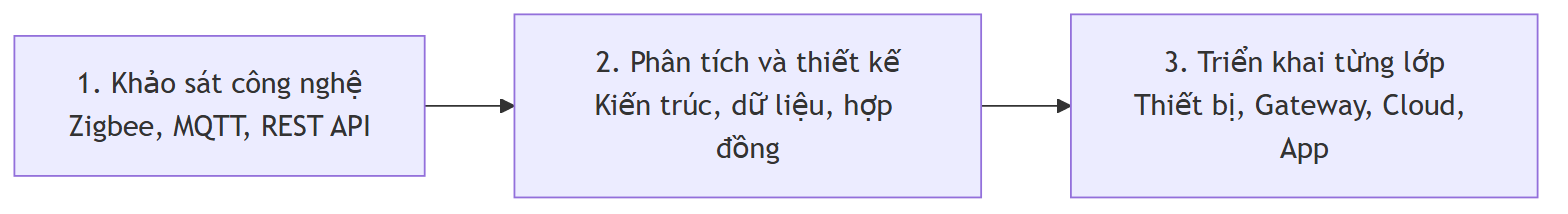
\includegraphics[width=0.82\textwidth]{Images/mermaid/ch1_project_method_1.png}\\[0.25cm]
    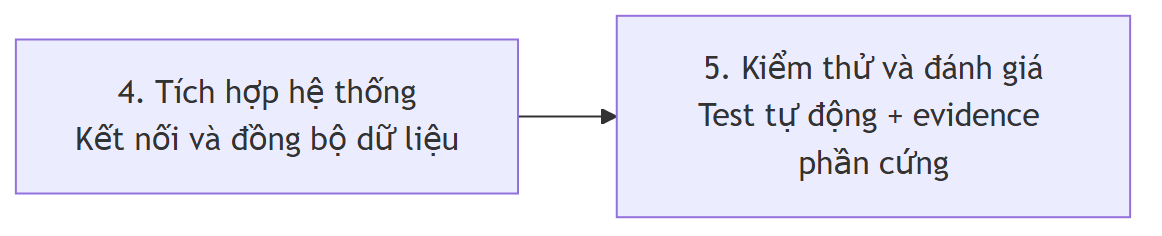
\includegraphics[width=0.58\textwidth]{Images/mermaid/ch1_project_method_2.png}
    \caption{Quy trình nghiên cứu và triển khai hệ thống}
    \label{fig:ch1-flowchart}
\end{figure}

Quy trình thực hiện bao gồm các giai đoạn cụ thể sau:

\textbf{Giai đoạn 1 -- Khảo sát và nghiên cứu công nghệ:} Nghiên cứu tài liệu kỹ thuật về chuẩn Zigbee 3.0, thư viện ZCL (Zigbee Cluster Library) của Silicon Labs, giao thức truyền thông MQTT và kiến trúc API hướng tài nguyên sử dụng REST.

\textbf{Giai đoạn 2 -- Thiết kế hệ thống:} Xác định sơ đồ khối kiến trúc hệ thống 4 lớp, thiết kế cấu trúc cơ sở dữ liệu PostgreSQL, xây dựng hợp đồng trao đổi bản tin MQTT (MQTT Contract JSON Schema) và cấu hình các topic phân cấp.

\textbf{Giai đoạn 3 -- Triển khai:} Lập trình firmware cho EFR32MG12; viết Z3Gateway bằng ngôn ngữ C; xây dựng Cloud API bằng FastAPI.

\textbf{Giai đoạn 4 -- Tích hợp hệ thống:} Kết nối Gateway host với chip NCP qua UART, kết nối Gateway lên Mosquitto Broker chạy trên container Docker, thiết lập liên kết đồng bộ giữa cơ sở dữ liệu và MQTT Client chạy nền trên Cloud.

\textbf{Giai đoạn 5 -- Kiểm thử và đánh giá:} Chạy các kịch bản kiểm thử tích hợp tự động bằng \text{pytest} cho backend và thực thi kiểm thử thủ công end-to-end trực tiếp trên phần cứng thật để thu thập log vận hành.

% ========================================
% 1.5 ĐÓNG GÓP CHÍNH CỦA ĐỒ ÁN
% ========================================
\section{Đóng góp chính của đồ án}
\label{sec:ch1-donggop}

Kết quả thực hiện đồ án mang lại một số đóng góp về kiến trúc tích hợp, quản lý lệnh, nhận dạng thiết bị và phương pháp kiểm thử. Bảng \ref{tab:ch1-donggop} tóm tắt các đóng góp và ý nghĩa kỹ thuật tương ứng.

\begin{table}[H]
\centering
\caption{Đóng góp chính và ý nghĩa kỹ thuật của đồ án}
\label{tab:ch1-donggop}
\begin{tabular}{|p{5.5cm}|p{9cm}|}
\hline
\textbf{Giải pháp phát triển} & \textbf{Ý nghĩa thực tế và kỹ thuật} \\ \hline
Kiến trúc Gateway C đơn tiến trình tích hợp MQTT client & Giữ đường xử lý command, report và event trong cùng ứng dụng Gateway, làm rõ trách nhiệm giữa MQTT callback, hàng đợi lệnh và Zigbee callback. \\ \hline
Mô hình theo dõi vòng đời lệnh điều khiển (Command Lifecycle) & Cho phép theo dõi tường minh trạng thái xử lý gói tin qua các pha (accepted, queued, sent, executed, failed, timeout), giải quyết bài toán lệnh bị treo hoặc mất gói vô tuyến mà cloud không phát hiện được. \\ \hline
Chuẩn hóa mô hình nhận dạng thiết bị qua \text{device\_id} logic & Tách biệt định danh cơ sở dữ liệu khỏi địa chỉ phần cứng cố định (EUI-64) hoặc địa chỉ động (16-bit nwk\_addr), tăng tính bảo mật và cho phép linh hoạt thay thế phần cứng lỗi. \\ \hline
Khung test case xuyên suốt và nguyên tắc evidence & Tách rõ kết quả test phần mềm đã có output với test phần cứng còn cần log, API response, ảnh hoặc video trước khi đánh giá. \\ \hline
\end{tabular}
\end{table}

Chương~\ref{ch:ketqua} trình bày output của các nhóm test phần mềm và chỉ rõ những test phần cứng còn thiếu evidence. Cách ghi nhận này giúp phân biệt phần đã kiểm chứng tự động với phần cần tiếp tục đo trên mô hình thực.

% ========================================
% 1.6 CẤU TRÚC BÁO CÁO
% ========================================
\section{Cấu trúc báo cáo}
\label{sec:ch1-cautruc}

Nội dung báo cáo đồ án tốt nghiệp được tổ chức thành 6 chương chính sau đây:

\textbf{Chương~\ref{ch:tongquan-detai} -- Tổng quan đề tài:} Giới thiệu bối cảnh, lý do chọn đề tài, xác định mục tiêu, phạm vi nghiên cứu, phương pháp thực hiện và cấu trúc tổng thể của báo cáo.

\textbf{Chương~\ref{ch:lythuyet} -- Cơ sở lý thuyết và công nghệ nền:} Trình bày nền tảng lý thuyết về giao thức mạng Zigbee, thư viện cluster ZCL, giao thức MQTT, giao tiếp nối tiếp UART/ASH và các kit vi điều khiển phần cứng được sử dụng.

\textbf{Chương~\ref{ch:thietke} -- Phân tích yêu cầu và thiết kế hệ thống:} Phân tích các yêu cầu chức năng, phi chức năng, xây dựng sơ đồ kiến trúc tổng thể, mô hình dữ liệu, đặc tả giao diện API và hợp đồng trao đổi bản tin MQTT Contract.

\textbf{Chương~\ref{ch:trienkhai} -- Triển khai hệ thống:} Trình bày chi tiết quá trình lập trình firmware thiết bị, viết ứng dụng Gateway C, lập trình Cloud Backend bằng FastAPI và giải quyết các lỗi thực tế khi deploy lên EC2.

\textbf{Chương~\ref{ch:ketqua} -- Kiểm thử và đánh giá:} Thiết lập kế hoạch kiểm thử, trình bày kết quả chạy các test case cụ thể, ghi nhận các bằng chứng logs/traces và phân tích ưu điểm cũng như hạn chế của hệ thống.

\textbf{Chương~\ref{ch:ketluan} -- Kết luận và hướng phát triển:} Tổng kết các kết quả có evidence, nêu kiến thức tích lũy và đề xuất các hướng mở rộng về độ ổn định, giám sát, bảo mật và cập nhật trạng thái gần thời gian thực.
